% =====================================================================
%  Chapter 2 -- Literature Review   (source: Literature_Review_Draft_v9.docx)
% =====================================================================
\chapter{Literature Review}
\label{ch:literature}
\edited{Section 2.3 restructured under three requirements (reliability, form
factor, efficiency), each comparing single-phase and phase-change cooling and
their implications for magnetic components. \Cref{tab:cooling-strategies} is
regrouped to match, with an added row for loss in magnetics.}

This chapter reviews the literature on cooling power electronic converters
(PECs) with liquid metal. It opens with the sources of loss in inductive power
transfer (IPT) systems, the application that motivates this work
(\cref{sec:ipt-losses}). It then presents the current trend that the power
density of PECs is increasing (\cref{sec:motivation}), and the reliability,
form-factor and efficiency requirements that their thermal management must meet,
which point to liquid metal cooling as a potential solution
(\cref{sec:thermal-management}). \Cref{sec:liquid-metal} evaluates this
proposal, and \cref{sec:research-gap} identifies the research gap and states
the research questions of this project.
\edited{The draft pointed to ``Section 2.6'' for the research gap; there is no
Section 2.6 (the gap is \cref{sec:research-gap}). All section, figure, table and
equation references are now generated with \texttt{\textbackslash cref}, so they
will stay correct if the structure changes.}

% ---------------------------------------------------------------------
\section{Thermal Losses in Inductive Power Transfer Systems}
\label{sec:ipt-losses}

IPT systems transfer power across a large air gap between loosely coupled
coils, and their losses are spread across the power electronics, the
compensation network and the magnetic pads. \Cref{fig:kim-losses} shows the
loss distribution that Kim \emph{et al.}\ measured and simulated for a
\SI{10}{\kilo\watt} IPT system with double-D (DD) pads, operating at
\SI{85}{\kilo\hertz} at a worst-case ambient temperature of
\SI{50}{\celsius}~\cite{kim_thermal_2022}. Most of the loss occurs in the pads,
chiefly in the Litz wire and ferrite, with smaller shares in the compensation
capacitors and in the aluminium shielding sheet, in which the leakage field
induces eddy currents. The inverter and rectifier dissipate about
\SIrange{70}{80}{\watt} each.

\begin{figure}[htbp]
  \centering
  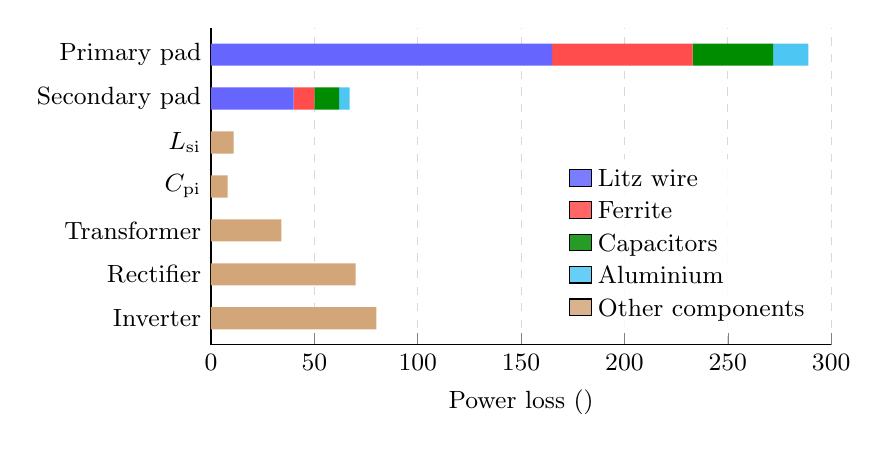
\begin{tikzpicture}
    \begin{axis}[
      xbar stacked,
      width=0.78\linewidth, height=5.6cm,
      bar width=8pt,
      xmin=0, xmax=300,
      xlabel={Power loss (\si{\watt})},
      symbolic y coords={Inverter,Rectifier,Transformer,Cpi,Lsi,Secondary,Primary},
      ytick=data,
      yticklabels={Inverter, Rectifier, Transformer, $C_{\mathrm{pi}}$,
        $L_{\mathrm{si}}$, Secondary pad, Primary pad},
      tick label style={font=\small},
      label style={font=\small},
      xmajorgrids=true, grid style={dashed, gray!30},
      axis x line*=bottom, axis y line*=left,
      enlarge y limits=0.1,
      legend style={at={(0.98,0.04)}, anchor=south east, font=\small,
        draw=none, fill=white, fill opacity=0.85, text opacity=1},
      legend cell align=left,
    ]
      \addplot[fill=blue!60, draw=none] coordinates
        {(0,Inverter) (0,Rectifier) (0,Transformer) (0,Cpi) (0,Lsi) (40,Secondary) (165,Primary)};
      \addplot[fill=red!70, draw=none] coordinates
        {(0,Inverter) (0,Rectifier) (0,Transformer) (0,Cpi) (0,Lsi) (10,Secondary) (68,Primary)};
      \addplot[fill=green!55!black, draw=none] coordinates
        {(0,Inverter) (0,Rectifier) (0,Transformer) (0,Cpi) (0,Lsi) (12,Secondary) (39,Primary)};
      \addplot[fill=cyan!70, draw=none] coordinates
        {(0,Inverter) (0,Rectifier) (0,Transformer) (0,Cpi) (0,Lsi) (5,Secondary) (17,Primary)};
      \addplot[fill=brown!70, draw=none] coordinates
        {(80,Inverter) (70,Rectifier) (34,Transformer) (8,Cpi) (11,Lsi) (0,Secondary) (0,Primary)};
      \legend{Litz wire, Ferrite, Capacitors, Aluminium, Other components}
    \end{axis}
  \end{tikzpicture}
  \caption{Power loss distribution across a \SI{10}{\kilo\watt},
    \SI{85}{\kilo\hertz} IPT system with DD pads at an ambient temperature of
    \SI{50}{\celsius}, recreated from Kim \emph{et al.}~\cite{kim_thermal_2022}
    (values read from the original figure). $L_{\mathrm{si}}$ and $C_{\mathrm{pi}}$
    are components of the compensation network.}
  \label{fig:kim-losses}
\end{figure}

These losses differ in density. The pad losses are spread over about
\SI{0.8}{\metre} by \SI{0.6}{\metre} inside a strong alternating magnetic field,
and the pad is cooled passively, reaching a simulated peak temperature of about
\SI{96}{\celsius}. Its components also change with temperature: the Litz wire
resistance rises by about \SI{0.4}{\percent} per degree and the ferrite loss
varies nonlinearly, so power loss and temperature cannot be considered
separately~\cite{kim_thermal_2022}. The semiconductor losses, by contrast, are
concentrated in small switching devices placed away from the coupler. Where an
alternative coolant could be used in an IPT system therefore depends on both the
heat flux and the magnetic field the cooling system is exposed to, a question this report
returns to in \cref{sec:disc-suitability}.

Wireless charging of light-duty electric vehicles is standardised at a nominal
operating frequency of \SI{85}{\kilo\hertz}~\cite{society_of_automotive_engineers_r_2024},
the frequency used by Kim \emph{et al.}~\cite{kim_thermal_2022} and by
high-power IPT systems for public transport~\cite{bosshard_multi-objective_2016}.
The magnetic components of these systems are driven at this frequency, so any
cooling hardware placed near them is exposed to leakage fields at this
frequency. For this reason,
the power-dense inductor used in this work (\cref{sec:inductor-design}) is
operated at \SI{85}{\kilo\hertz}.
\issue{The Zotero record for SAE J2954 (\texttt{society\_of\_automotive\_engineers\_r\_2024})
has typos in its title (``J2594'', ``Vechicles''), which will print in the
reference list. Fix them in Zotero and re-export the bib file.}

% ---------------------------------------------------------------------
\section{Power Density in Power Electronic Converters}
\label{sec:motivation}

PECs switch semiconductor devices at high frequency and use passive components,
chiefly inductors, transformers and capacitors, to store and release energy in
each switching cycle and to filter the resulting
waveforms~\cite{morroni_understanding_2023}. Magnetic components, frequently the
largest passive devices, are difficult to scale and often restrict the
achievable power
density~\cite{biela_cooling_2007,morroni_understanding_2023,sullivan_size_2016};
with heat sinks, they account for the largest portion of a power solution's
size~\cite{biela_cooling_2007,morroni_understanding_2023}. Higher switching
frequencies, now practical with wide-bandgap devices~\cite{gao_modeling_2022},
permit smaller passive components because less energy is stored per
cycle~\cite{morroni_understanding_2023}, but losses limit this gain.

Friedli \emph{et al.}\ demonstrated this trade-off with \SI{10}{\kilo\watt}
rectifiers built for switching frequencies from \SI{72}{\kilo\hertz} to
\SI{1}{\mega\hertz}~\cite{friedli_essence_2014}. As the frequency rose, the
boost inductor shrank, but the efficiency fell almost linearly from
\SI{97.3}{\percent} to \SI{93}{\percent} as the switching losses grew. With
forced-air cooling, the growing heat sink cancelled the gain, so the power
density peaked at \SI{6.5}{\kilo\watt\per\deci\metre\cubed} near
\SI{350}{\kilo\hertz}, and \SI{1}{\mega\hertz} could not be air-cooled at all.
Only with water cooling did the power density keep rising, to
\SI{14.1}{\kilo\watt\per\deci\metre\cubed} at
\SI{1}{\mega\hertz}~\cite{friedli_essence_2014}. The cooling method therefore
sets the achievable power density, and as shrinking components raise the heat
flux~\cite{morroni_understanding_2023}, further size reduction requires cooling
methods that transfer more heat per unit area~\cite{biela_cooling_2007}.

% ---------------------------------------------------------------------
\section{Thermal Management of Power Electronic Converters}
\label{sec:thermal-management}

The thermal management of a power-dense PEC must meet three requirements. It
must keep the converter reliable, fit within its form factor, and do so
efficiently, without adding significant loss to the converter, including in
nearby magnetic components. The following sections consider each requirement
in turn, comparing the two established families of cooling: single-phase
cooling with air or water, and phase-change cooling by boiling or heat pipes.
\Cref{tab:cooling-strategies} summarises how each meets these
requirements~\cite{liu_thermal_2025,rahman_emerging_2024,laloya_heat_2016,mudawar_assessment_2001}.

\begin{table}[htbp]
  \centering
  \caption[Thermal management requirements and established cooling strategies]{Summary
    of how established cooling strategies meet the requirements for PEC thermal
    management. COP: coefficient of performance, the ratio of heat removed to
    cooling power consumed.}
  \label{tab:cooling-strategies}
  \small
  \begin{tabularx}{\linewidth}{@{}>{\raggedright\arraybackslash}p{3.0cm} L L@{}}
    \toprule
    Requirement & Single-phase (air, water) & Phase change (boiling, heat pipes) \\
    \midrule
    \multicolumn{3}{@{}l}{\textit{Reliability}} \\
    \quad Maximum temperature
      & Forced air: tens of \si{\watt\per\centi\metre\squared};
        water cold plate: hundreds of \si{\watt\per\centi\metre\squared};
        water microchannel: $\approx$\SI{1000}{\watt\per\centi\metre\squared}
      & Highest, but capped by CHF \\
    \quad Temperature swing
      & Fan speed or flow rate provides control input
      & Boiling-onset thermal shock; no control input when passive \\
    \addlinespace
    \multicolumn{3}{@{}l}{\textit{Form factor}} \\
    \quad Compactness
      & Air: bulky heat sink; water: compact at the device, pump and radiator remote
      & Smaller and lighter than single-phase \\
    \addlinespace
    \multicolumn{3}{@{}l}{\textit{Efficiency}} \\
    \quad Burden power
      & Fans (COP 10--100) or pump (COP 300--500); rises steeply as channels narrow
      & Low; often passive \\
    \quad Loss in magnetics
      & \multicolumn{2}{>{\raggedright\arraybackslash}p{0.62\linewidth}}{Any
        conductive cooling hardware in a leakage field incurs eddy-current loss} \\
    \bottomrule
  \end{tabularx}
\end{table}

\subsection{Reliability Requirement}
\label{sec:reliability}

Thermal management is required, above all, to keep increasingly power-dense
PECs reliable. Thermal stress causes over \SI{50}{\percent} of electronic
equipment failures~\cite{rahman_emerging_2024}, and power semiconductors, which
dominate the overall reliability of power converters, account for approximately
\SI{31}{\percent} of PEC failures~\cite{kalay_systematic_2025}. The
Coffin--Manson model relates the number of thermal cycles to failure of a
semiconductor device to its junction temperature
swing~\cite{kalay_systematic_2025,albarbar_thermal_2018}:
\begin{equation}
  N_{\mathrm{f}} = \alpha \left(\Delta T_{\mathrm{j}}\right)^{\beta},
  \label{eq:coffin-manson}
\end{equation}
where $N_{\mathrm{f}}$ is the number of power cycles (in thousands) to failure,
$\Delta T_{\mathrm{j}}$ is the junction temperature swing, and $\alpha$ and
$\beta$ are experimentally determined parameters~\cite{kalay_systematic_2025}.
This simplified form omits the absolute-temperature term, which becomes
significant mainly above about \SI{200}{\celsius}~\cite{kalay_systematic_2025}.
Magnetic components also fail under thermal
stress~\cite{biela_cooling_2007,mengesha_advanced_2025,li_review_2022,lawton_power_2024}.
For reliability, the cooling system must therefore hold the maximum temperature
of both semiconductors and magnetics below their operating limits, and suppress
the temperature swing.

Single-phase cooling meets both requirements to a degree. Natural convection,
the simplest scheme, is limited by the low heat transfer coefficient of
air~\cite{biela_cooling_2007}, and is the conventional way of cooling magnetic
components from their exposed surfaces. Gao \emph{et al.}'s passively cooled
planar inductor rose more than \SI{65}{\celsius} in temperature at
\SI{12}{\ampere} rms, whereas with an engineered conduction path to a
liquid-cooled cold plate (\cref{fig:gao-inductor}) the rise was less than
\SI{3}{\celsius}~\cite{gao_modeling_2022}. Forced air and liquid cooling raise
the achievable heat flux, and their fan speed or flow rate provides a control
input over the temperature swing. Their heat flux, however, is bounded by the
coolant~\cite{rahman_emerging_2024,laloya_heat_2016}. Phase-change cooling
absorbs latent heat and offers the highest heat
flux~\cite{laloya_heat_2016,mudawar_assessment_2001}. Above the critical heat
flux (CHF), however, vapour blocks liquid access to the surface and the device
temperature rises uncontrollably. CHF is difficult to predict, so the safety
margin it demands erodes this advantage~\cite{mudawar_assessment_2001}, and
passive phase-change schemes offer no control over the temperature swing.

\begin{figure}[tbp]
  \centering
  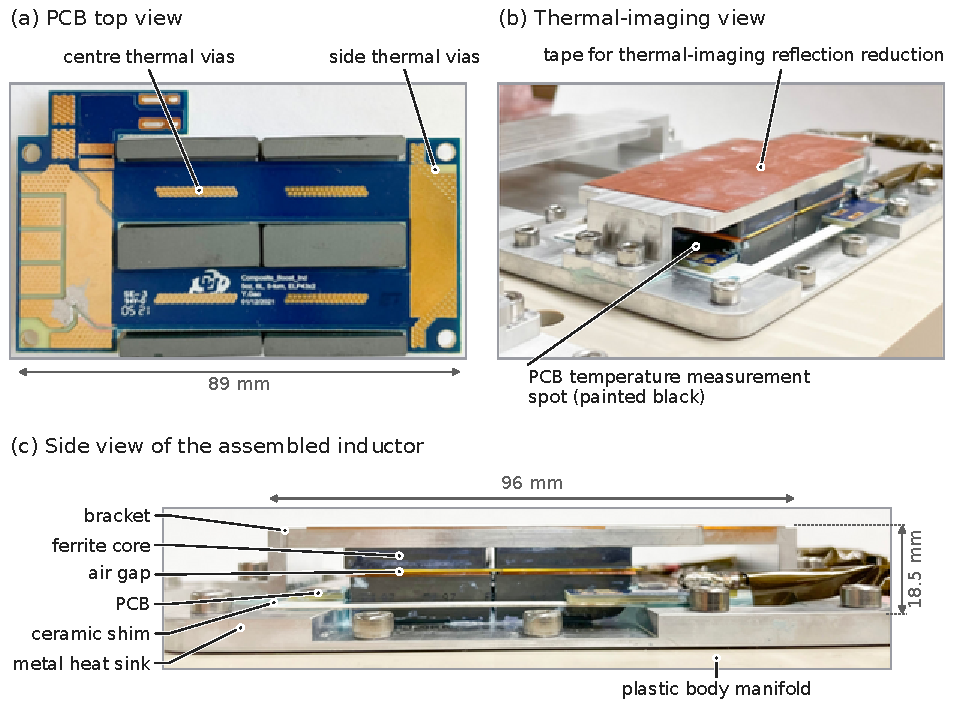
\includegraphics[width=0.75\linewidth]{gao_inductor_prototype}
  \caption[Planar inductor prototype of Gao \emph{et al.}]{Planar inductor
    prototype of Gao \emph{et al.} with an engineered conduction path to the
    cold plate: (a)~PCB top view; (b)~view used for thermal imaging;
    (c)~side view of the assembled inductor. Adapted
    from~\cite{gao_modeling_2022}.}
  \label{fig:gao-inductor}
\end{figure}

\subsection{Form Factor Requirement}
\label{sec:form-factor}

The cooling system must not erode the power density it is meant to enable. With
the magnetic components, heat sinks account for the largest portion of a power
converter's size, and in compact converters the thermal management system can
occupy a large share of the
volume~\cite{biela_cooling_2007,morroni_understanding_2023,friedli_essence_2014}.
Air cooling requires bulky heat sinks, which limited the power density of the
rectifiers of Friedli \emph{et al.}\ (\cref{sec:motivation}). Water cooling is
compact at the device, as the pump and radiator can be placed
remotely~\cite{friedli_essence_2014,laloya_heat_2016}, while phase-change
systems can be smaller and lighter still~\cite{laloya_heat_2016}. For magnetic
components, a compact cooling system must be placed as close as possible to the
windings, typically on both the top and bottom of the
core~\cite{krismer_accurate_2010,biela_cooling_2007}, which places it directly in
the component's leakage field.

\subsection{Efficiency Requirement}
\label{sec:efficiency-req}

To retain the efficiency of the converter, the power drawn by the cooling system,
its burden power, must remain small relative to the power
processed~\cite{laloya_heat_2016}, and the cooling hardware must not introduce
excessive loss into the converter. Single-phase cooling requires fans or pumps,
and raising its heat flux requires narrower channels, which raise the pressure
drop and pumping power steeply~\cite{rahman_emerging_2024,laloya_heat_2016}.
Single-phase cooling therefore trades the maximum temperature it can hold
against the burden power it draws. Phase-change cooling draws little or no
burden power, and is often passive~\cite{laloya_heat_2016}.

Cooling hardware placed near magnetic components, whether single-phase or
phase-change, sits in their leakage field and suffers eddy-current
loss~\cite{biela_cooling_2007,gao_modeling_2022,ouyang_overview_2014}. In Gao
\emph{et al.}'s design, the cold plate and bracket raised the measured AC winding
resistance by \SI{34}{\percent}~\cite{gao_modeling_2022}, and the aluminium
shielding sheet of an IPT pad dissipates about \SI{17}{\watt} in the same way
(\cref{fig:kim-losses})~\cite{kim_thermal_2022}. Biela and Kolar similarly found
that heat-transfer components near an inductor air gap must be recessed from
it~\cite{biela_cooling_2007}. Because magnetic components are present in most
converters~\cite{morroni_understanding_2023}, their leakage fields must be
considered in any PEC cooling design, even where the magnetics are not the main
thermal constraint.

No established scheme therefore meets all three requirements. Phase-change
cooling offers the highest heat flux at low burden power, but is capped by CHF
and offers no control over the temperature swing when passive. Single-phase
cooling is controllable, but its heat flux is bounded by the low thermal
conductivity of air and water, so a higher heat flux costs pumping power. A
coolant with substantially higher thermal conductivity could ease this trade-off
while keeping flow-rate control, which motivates much of the research into
liquid metal coolants~\cite{hodes_potential_2014}.

% ---------------------------------------------------------------------
\section{Liquid Metal as a Coolant}
\label{sec:liquid-metal}

Liquid metals have long been used as coolants where heat fluxes and operating
temperatures exceed those that conventional fluids can tolerate~\cite{rowinski_small_2015}. 
Much of the early characterisation of liquid metal cooling systems was carried out as fundamental research for nuclear
reactors~\cite{rowinski_small_2015}. These systems typically use lead or sodium
coolants, but lead is toxic and requires careful handling and
containment~\cite{oecd_handbook_2015}, whereas sodium is highly chemically
reactive, particularly with water and air, posing fire and explosion
hazards~\cite{foust_sodium-nak_1972}. These factors complicate broader commercial
deployment.

Liquid metal has more recently been proposed as a coolant for computing hardware and
PECs~\cite{fan_ultra-efficient_2026,zhang_water-based_2015}. The driving factor is its high thermal
conductivity, which promises high heat transfer rates~\cite{hodes_potential_2014,fan_ultra-efficient_2026,zhang_experimental_2019,zhang_investigation_2023}.
Such applications typically use gallium (Ga)-based eutectic alloys, the most
common being Galinstan (GaInSn), which is non-toxic and remains liquid at room temperature~\cite{hodes_potential_2014,an_liquid_2024}. 
Galinstan has a thermal conductivity of \SI{16.5}{\watt\per\metre\per\kelvin},
approximately 28 times that of water (\cref{tab:galinstan-properties}), which
enhances heat spreading and reduces temperature gradients~\cite{hodes_potential_2014,zhang_experimental_2019}. 
A Galinstan loop offers single-phase cooling, with no boiling limit to design around, and has the potential to
remove a higher heat flux than water~\cite{hodes_potential_2014, zhang_experimental_2019}.

These benefits come with significant trade-offs (\cref{tab:galinstan-properties}).
High density and viscosity raise pumping power and system weight. Because the
volumetric heat capacity is low, more than twice the flow of water is needed
for the same coolant temperature rise. Electrical conductivity rules out direct
contact with live parts and exposes the coolant to induction heating. 
The wide liquid range, by contrast, removes the CHF limit that
constrains phase-change cooling. The material cost is high, but at the
system level water and Galinstan are comparable because water pumps are
expensive~\cite{fan_ultra-efficient_2026}. Kwon~\cite{kwon_project_2025}
therefore concluded that liquid metal suits specialised applications where
efficiency, compactness and reliability justify its cost.

\begin{table}[htbp]
  \centering
  \caption{Selected properties and cost of the Galinstan used in this work
    (Rich Metals grade EU-10C, 68.5Ga--21.5In--10Sn by
    weight~\cite{noauthor_gainsn_nodate}) relative to water.}
  \label{tab:galinstan-properties}
  \small
  \begin{tabularx}{\linewidth}{@{}>{\raggedright\arraybackslash}p{3.2cm}
      >{\raggedright\arraybackslash}p{2.9cm} L >{\raggedright\arraybackslash}p{1.3cm}@{}}
    \toprule
    Property & Galinstan & Relative to water & Source \\
    \midrule
    Thermal conductivity & \SI{16.5}{\watt\per\metre\per\kelvin} & About 28 times higher & \cite{noauthor_gainsn_nodate} \\
    Density & \SI{6370}{\kilogram\per\metre\cubed} & More than six times higher & \cite{noauthor_gainsn_nodate} \\
    Dynamic viscosity & \SI{2}{\milli\pascal\second} & About 2 times higher & \cite{noauthor_gainsn_nodate} \\
    Specific heat capacity & \SI{366}{\joule\per\kilogram\per\kelvin} & About one-fourteenth & \cite{zhang_experimental_2019} \\
    Volumetric heat capacity & \SI{2.3}{\mega\joule\per\metre\cubed\per\kelvin} & 0.45 times, so about 2.2 times the flow for equal $\Delta T$ & \cite{noauthor_gainsn_nodate} \\
    Electrical conductivity & \SI{3.46e6}{\siemens\per\metre} & Conductor (deionised water: \SI{5.5e-6}{\siemens\per\metre}) & \cite{noauthor_gainsn_nodate} \\
    Melting and boiling points & \SI{10}{\celsius} and above \SI{1300}{\celsius} & Liquid above \SI{10}{\celsius}, so it can solidify in cold storage; boiling will not occur & \cite{noauthor_gainsn_nodate,hodes_potential_2014} \\
    Material cost & US\$200--2000/kg & Orders of magnitude higher & \cite{an_liquid_2024} \\
    \bottomrule
  \end{tabularx}
\end{table}

Much of the reviewed work on Galinstan and other Ga-based coolants focuses on
micro- and mini-channel heat sinks for electronics, typically for heat loads
from watts to hundreds of watts. It is unclear from the literature whether such
systems can be scaled up to the channel sizes and temperatures more typical of
PECs. For example, EV-charging PECs have power classes on the order of tens of
kilowatts for light-duty vehicles and are being standardised up to
\SI{1}{\mega\watt} for heavy-duty
vehicles~\cite{lawton_power_2024,liu_thermal_2025,abb_e-mobility_mcs1200_nodate}. Large liquid
metal systems have been realised for nuclear reactors~\cite{rowinski_small_2015},
but these use different metals, operate at much higher temperatures and are much
larger than even the most powerful PEC applications, although some work has
addressed power electronic
converters~\cite{fan_ultra-efficient_2026,fan_liquid_2021}.

% ---------------------------------------------------------------------
\subsection{Electromagnetic Pumping}
\label{sec:em-pumping}

The low volumetric heat capacity of Galinstan makes pumping demanding. For a
heat load $Q$ and coolant temperature rise $\Delta T$, the required volumetric
flow rate is
\begin{equation}
  \Vdot = \frac{Q}{\rho \, \cp \, \Delta T},
  \label{eq:flow-requirement}
\end{equation}
where $\rho$ is the coolant density and $\cp$ its specific heat capacity.
Galinstan therefore needs about 2.2 times the flow of water
(\cref{tab:galinstan-properties}), which is identified as the primary
bottleneck for liquid metal heat sinks~\cite{hodes_potential_2014,an_liquid_2024}.
Its high thermal conductivity partly offsets this, because it sustains high heat
transfer coefficients in wider channels with a lower pressure
drop~\cite{zhang_water-based_2015,an_liquid_2024}.

The electrical conductivity of Galinstan also allows it to be driven by
electromagnetic (EM) pumps with no moving parts, which are silent,
vibration-free and compact~\cite{hodes_potential_2014}. Previous Part~IV
projects used a permanent-magnet DC conduction
pump~\cite{kwon_project_2025,loh_project_2025}. In this pump, a current $I$
passed through the coolant perpendicular to a magnetic field of flux density
$B$ produces a Lorentz force density
$\mathbf{J}\times\mathbf{B}$~\cite{kwon_project_2025}. An approximation for the
pressure developed is
\begin{equation}
  \Delta p = \frac{B I}{h},
  \label{eq:mhd-pressure}
\end{equation}
where $h$ is the channel height parallel to
$\mathbf{B}$~\cite{loh_project_2025}. Pressure therefore scales directly with
current, so the flow can be modulated to suppress temperature
swing~\cite{an_liquid_2024}, and shallow channels with strong magnets are
favoured. The cost is operation at high current and low voltage
(\SIrange{1}{100}{\ampere}, \SIrange{0.01}{0.5}{\volt},
\SIrange{0.1}{50}{\watt}), with efficiencies of only about
\SIrange{6}{10}{\percent}~\cite{an_liquid_2024,hodes_potential_2014}. Even
so, a conduction pump has drawn less than \SI{15}{\percent} of the power of a
mechanical water pump for the same cooling performance~\cite{an_liquid_2024}.

Induction pumps instead induce current in the coolant through an alternating or
travelling field. They are larger and more complex, but they develop greater
force~\cite{an_liquid_2024}. The field can also come from the converter itself.
Fan \emph{et al.}\ integrated an MHD pump into an inductor, so that the flow
self-adjusts with converter load~\cite{fan_liquid_2021}. The cost is
eddy-current losses in the coolant~\cite{fan_ultra-efficient_2026}. EM pumps
are, however, generally reported as individual designs. Among liquid metal
systems developed for power electronics, only those of Fan
\emph{et al.}\ have been compared against an equivalent water
system~\cite{fan_liquid_2021,fan_ultra-efficient_2026}.

% ---------------------------------------------------------------------
\subsection{Compatibility with Electrical Equipment}
\label{sec:compatibility}

Commercial use of Galinstan raises three concerns: material safety, corrosion
and electromagnetic compatibility. Galinstan was developed as a non-toxic,
non-flammable replacement for mercury. Its negligible vapour pressure means it
poses no inhalation risk~\cite{hodes_potential_2014}. Gallium oxide can damage
the respiratory system at high airborne concentrations, but a closed loop
releases only minimal amounts~\cite{an_liquid_2024}. Prior prototypes managed
skin contact and spillage with gloves, eye protection and containment
trays~\cite{kwon_project_2025,loh_project_2025}.

Ga-based alloys corrode aluminium severely, and copper requires protection
above \SI{100}{\celsius}~\cite{an_liquid_2024}. Erosion at high flow velocities
and the effect on ductile metals remain unstudied~\cite{hodes_potential_2014}.
Plastics and nickel-plated metals~\cite{hodes_potential_2014}, as well as
ceramics such as aluminium nitride~\cite{an_liquid_2024}, are compatible.
Aluminium nitride is also both thermally conductive and electrically
insulating, though expensive~\cite{gao_modeling_2022}.

Electrically, the coolant is a conductor. A leak onto
energised circuitry is a direct short~\cite{hodes_potential_2014}. The loop also
galvanically connects every wetted part, so the EM pump supply can energise the
radiator and cold plate~\cite{kwon_project_2025}. There is also potential for nearby
magnetics to induce eddy currents in the coolant, though this has not been strictly explored in the literature
(\cref{sec:thermal-management})~\cite{an_liquid_2024, fan_ultra-efficient_2026}.
As a result, low-cost plastic piping suits low-field regions. 
Near magnetics, it may be preferable to shield the coolant with a more conductive material to reduce eddy losses.

% ---------------------------------------------------------------------
\section{Research Gap and Objectives}
\label{sec:research-gap}

\subsection{Research Gap}
\edited{Trimmed only. The two opening sentences (water cooling is bounded by
water's thermal conductivity; Galinstan's higher conductivity can improve heat
transfer, both cited to Hodes \emph{et al.}) repeated
\cref{sec:thermal-management,sec:liquid-metal} and were cut. The two closing
sentences of the second gap (most converters contain magnetics; a cooling
system that does not cool them must still tolerate their leakage fields) are
now made in \cref{sec:thermal-management} and are replaced by a back-reference.
In the first gap, ``which use different metals at much higher temperatures''
was cut, as \cref{sec:liquid-metal} already says so.}

This study aims to address two gaps identified in the literature.

The first is the lack of comparisons between water and liquid metal at the scale
of a converter's cooling loop. Most existing comparisons are made for micro- and
mini-channel heat
sinks~\cite{hodes_potential_2014,zhang_water-based_2015,zhang_experimental_2019,an_liquid_2024},
or lie at the scale of nuclear reactors~\cite{rowinski_small_2015}. This study
aims to quantify the
trade-offs of the Galinstan system (as designed
in~\cite{kwon_project_2025,loh_project_2025}) relative to a comparable water-cooling
system.

The second is the cooling of magnetic components with Galinstan. To the author's
knowledge, no study has demonstrated Galinstan cooling of a magnetic component,
such as a power-dense inductor, or quantified the eddy-current losses induced in
the coolant by its leakage field. Eddy-current losses have been assessed in AC
conduction pumps~\cite{fan_ultra-efficient_2026}, and an inductor has been used to drive a
pump~\cite{fan_ultra-efficient_2026,fan_liquid_2021}, but not to cool the inductor itself
directly. As argued in \cref{sec:thermal-management}, the coolant's loss in a
leakage field matters even where the coolant does not cool the magnetics.

This project addresses both gaps using the existing Galinstan loop of
Loh~\cite{loh_project_2025} and Kwon~\cite{kwon_project_2025}. The loop comprises a
permanent-magnet MHD pump, perfluoroalkoxy (PFA) tubing, a cold plate and a
fan-cooled radiator, and can remove up to a \SI{72}{\watt} resistive
load~\cite{kwon_project_2025,loh_project_2025}. The loop was not tested against water
in the same apparatus, and its experiments did not consider magnetics:
Loh~\cite{loh_project_2025} focused on switching devices because Galinstan was
unlikely to interfere with them, unlike magnetics, and Kwon~\cite{kwon_project_2025}
excluded direct integration and testing with magnetics because of time
limitations and uncertainty about electromagnetic interference. Both recommended
comparison with water cooling, and Kwon also recommended testing higher heat
loads and investigating the interaction with inductive pad
fields~\cite{kwon_project_2025,loh_project_2025}.
\edited{``This project was not tested against water'' referred to the previous
project's loop, not this project; reworded to ``The loop was not tested
\dots''.}

\subsection{Research Questions}
\label{sec:research-questions}

These gaps lead to two research questions.

\begin{description}[leftmargin=3.2em,labelwidth=2.6em,labelsep=0.6em,itemsep=4pt]
    \item[RQ1] At the same heat load, how do the thermal resistance and pumping
    power of the Galinstan loop compare with those of a similar conventional
    water loop?
    \item[H1] Galinstan's higher thermal conductivity will lower the convective
    resistance relative to water in the same cold plate. However, the total
    thermal resistance of the Galinstan loop will be higher than that of the
    water loop. Its low volumetric heat capacity and low flow rate give a
    caloric resistance comparable to the conduction resistance of the cold
    plate.
    \item[RQ2] Can the Galinstan loop cool a power-dense inductor while adding
    minimal loss to the existing aluminium cold plate, and how large is the
    eddy-current loss induced in the coolant?
    \item[H2] The Galinstan loop will have a cooling effect on the inductor above that of natural convection. 
    The increase in loss due to eddy-current loss induced in the coolant will be
    small compared to the loss of introducing the cold plate.
    The metal of the cold plate between the inductor and the coolant is
    several skin depths thick at \SI{85}{\kilo\hertz}. Additionally, the high-frequency field will not change the coolant flow
    measurably. 
\end{description}
